
\begin{landscape}% Landscape page
\chapter{List of Phonemes and Features}
\begin{table}
\centering % Center table
\tiny
\begin{tabular}{|c|c|c|c|c|c|c|c|c|c|c|c|c|c|c|c|c|c|c|c|c|c|c|c|c|c|}
\hline

&\multicolumn{21}{|c|}{Features}\\
\hline
&	a	&	e	&	o	&	i	&	u	&	n	&	m	&	l	&	j	&	f	&	v	&	s	&	z   & \textipa{S}	&	\textipa{Z}	&	p	&	b	&	t	&	d	&	k	&	g	\\
\hline

$sonorant$	&	+	&	+	&	+	&	+	&	+	&	+	&	+	&	+	&	+	&	-	&	-	&	-	&	-	&	-	&	-	&	-	&	-	&	-	&	-	&	-	&	-	\\
$vowel$	&	+	&	+	&	+	&	+	&	+	&	-	&	-	&	-	&	-	&	-	&	-	&	-	&	-	&	-	&	-	&	-	&	-	&	-	&	-	&	-	&	-	\\
$nasal$	&	-	&	-	&	-	&	-	&	-	&	+	&	+	&	-	&	-	&	-	&	-	&	-	&	-	&	-	&	-	&	-	&	-	&	-	&	-	&	-	&	-	\\
$approximant$	&	-	&	-	&	-	&	-	&	-	&	-	&	-	&	+	&	+	&	-	&	-	&	-	&	-	&	-	&	-	&	-	&	-	&	-	&	-	&	-	&	-	\\
$fricative$	&	-	&	-	&	-	&	-	&	-	&	-	&	-	&	-	&	-	&	+	&	+	&	+	&	+	&	+	&	+	&	-	&	-	&	-	&	-	&	-	&	-	\\
$plosive$	&	-	&	-	&	-	&	-	&	-	&	-	&	-	&	-	&	-	&	-	&	-	&	-	&	-	&	-	&	-	&	+	&	+	&	+	&	+	&	+	&	+	\\
labial	&	-	&	-	&	-	&	-	&	-	&	-	&	+	&	-	&	-	&	+	&	+	&	-	&	-	&	-	&	-	&	+	&	+	&	-	&	-	&	-	&	-	\\
coronal	&	-	&	-	&	-	&	-	&	-	&	-	&	-	&	+	&	-	&	-	&	-	&	+	&	+	&	+	&	+	&	-	&	-	&	+	&	+	&	-	&	-	\\
dorsal	&	-	&	-	&	-	&	-	&	-	&	-	&	-	&	-	&	+	&	-	&	-	&	-	&	-	&	-	&	-	&	-	&	-	&	-	&	-	&	+	&	+	\\
alveolar	&	-	&	-	&	-	&	-	&	-	&	+	&	-	&	+	&	-	&	-	&	-	&	+	&	+	&	-	&	-	&	-	&	-	&	+	&	+	&	-	&	-	\\
palatal	&	-	&	-	&	-	&	-	&	-	&	-	&	-	&	-	&	+	&	-	&	-	&	-	&	-	&	+	&	+	&	-	&	-	&	-	&	-	&	-	&	-	\\
velar	&	-	&	-	&	-	&	-	&	-	&	-	&	-	&	-	&	-	&	-	&	-	&	-	&	-	&	-	&	-	&	-	&	-	&	-	&	-	&	+	&	+	\\
\hline

\end{tabular}
\caption{List of consonant and vowels in the experiment}
\end{table}
\end{landscape}


\begin{figure}[H]
\vspace{.3in}
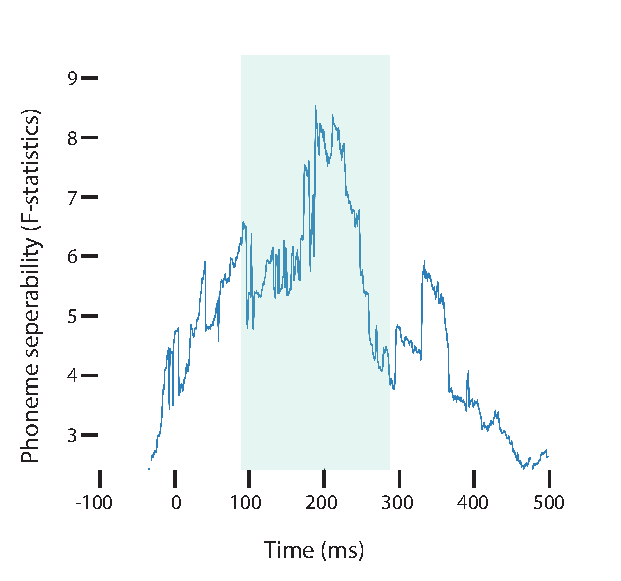
\includegraphics[width=\linewidth]{Figures/Ch3/Figure1_new.eps}
\caption{Optimal integration window: F-statistic for a running window of 200ms, averaged across units. Time values represent the center of the time window. We determined the optimal integration window (shaded area) according to the peak.}
\end{figure}